\chapter{Introduction}
	\label{chap:intro}

Over the past 10 years, deep neural networks have advanced tremendously, and have been used for safety and security-critical tasks, such as face recognition \cite{face_recognition}, self-driving cars \cite{self_driving_cars} and malware detection \cite{malware_detection}. However, neural networks are vulnerable to a variety of attacks which enable malicious agents to manipulate their outputs or leak information \cite{deep_leakage, trojan_attacks, poisoning_attacks, szegedy2014intriguing}. Adversarial attacks are one such class of attacks. First discovered in 2014 by Szegedy \textit{et al.} \cite{szegedy2014intriguing}, they involve crafting special perturbations that are added to the original input to make the victim model predict a wrong label. Moreover, these perturbations are often imperceptible to humans \cite{szegedy2014intriguing} and can fool a model into outputting specific wrong labels which are very different to the ground truth.

Since then, researchers have proven that attacks in the physical world \cite{evtimov_road_signs} and in cyberspace \cite{papernot_cyberspace_attack} are possible. For example, Eykholt \textit{et al.} \cite{evtimov_road_signs} successfully performed an adversarial attack that fooled a road sign recognition model in real life. Athalye \textit{et al.} \cite{athalye} created physical 3D objects that consistently fool neural networks for object recognition, regardless of the camera angle. This was in contrast to traditional attacks that create 2D adversarial images, as those are much less effective when printed and physically held in front of a camera \cite{lu_physical_experiments}. Consequently, the existence of adversarial examples undermines the safety of neural networks, and thus their applicability in safety or security-critical systems.

One disadvantage of the physical world attacks created in \cite{athalye} and \cite{evtimov_road_signs} is that they are \textbf{white-box} attacks, they require access to the victim model. This is necessary because they rely on gradient-descent optimisation and thus need to differentiate through the victim model. Another line of research looked at \textbf{black-box} attacks, which do not have this requirement \cite{akhtar} and are thus more practical for the attackers. However, the black-box attacks in the literature only create 2D adversarial examples in the lab setting and are less effective in a physical scenario.

An adversarial attack that is both black-box and applicable to the physical domain would be especially practical for attackers. Therefore, my project will try to combine the framework used in Athalye \textit{et al.} \cite{athalye} and the generative model presented in \cite{zheng_black_box_GAN} to create a black-box adversarial attack. It which produces 3D rendered objects that can consistently fool object classifier neural networks. The findings may be useful for understanding adversarial attacks further and for creating better defence methods.

\section{Motivation}
    \label{sec:motivation}
	
Adversarial attacks are often highly effective at fooling a victim model \cite{akhtar, silva_survey, dong2020benchmarking, robustart, fgsm}. Hendrik Metzen \textit{et al.} \cite{Metzen_2017_ICCV} attacked an image segmentation neural network used in a self-driving car. They managed to make the victim model not perceive pedestrians, as 84.5\% of pixels making up pedestrians were misclassified. If an attacker were to implement this in real life, the self-driving car could have run over pedestrians, because it would not see them, as figure \ref{fig:adversarial_segmentation} on page \pageref{fig:adversarial_segmentation} shows. Therefore, adversarial examples are a threat to neural networks used in safety-critical systems.

\begin{figure}[ht]
    \centering
    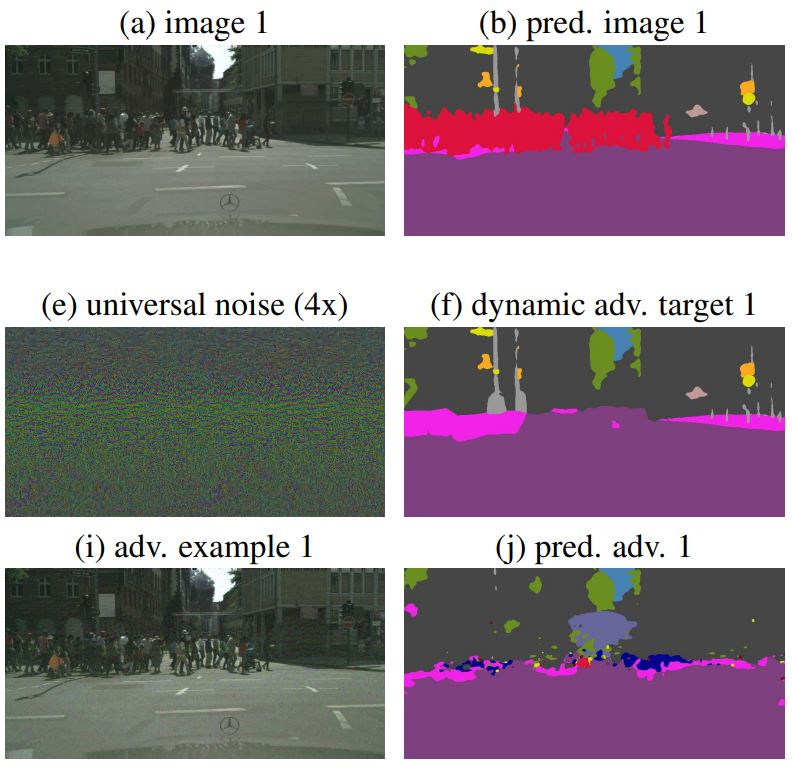
\includegraphics[width=0.75\textwidth]{graphics/adversarial_segmentation.JPG}
    \caption[Example of an adversarial example against neural network used in self-driving car.]{Example of an adversarial attack which removes pedestrians from a scene, as perceived by a neural network. The top row contains the original image and the correct image segmentation. The middle row shows the adversarial noise and the target segmentation, which has the pedestrians removed from the scene. The last row shows the adversarial example and the predicted segmentation. Taken from \cite{Metzen_2017_ICCV}.}
    \label{fig:adversarial_segmentation}
\end{figure}

Most attacks, including the one in figure \ref{fig:adversarial_segmentation}, directly add the image perturbations to the whole input image. In a realistic setting, the attacker would not be able to directly manipulate the input to a neural network, especially when the neural network takes its input from sensors. Examples include robots and self-driving cars which use cameras and voice command systems. On the other hand, Eykholt \textit{et al.} \cite{evtimov_road_signs} created adversarial patches which were stuck over a real STOP road sign. They then took pictures of the sign from a moving car and found that they were misclassified 84.8 and 87.5\% of the time by two different neural networks, respectively. Their attack would have made a self-driving car not stop at an intersection, and potentially cause a car crash.

The attacks against cyber-physical systems presented in \cite{athalye} and \cite{evtimov_road_signs} are \textbf{white-box}, they require access to the victim model's architecture and parameters. Traditional security measures such as encryption and network access control could secure the model and prevent attacks. But \textbf{black-box} attacks do not need access to the victim, thus bypassing those security measures. Consequently, they are more likely to be used by malicious agents. 

Therefore, black-box attacks which also work in physical settings are the attacks most likely to be used by malicious agents. However, to my knowledge, no attack in the literature has both of these characteristics. The black-box attacks in \cite{upset_angri, zheng_black_box_GAN, advGAN} only create adversarial noise for 2D images. The purpose of this project is to create a generative model for creating 3D adversarial objects \cite{athalye} and see if it is effective.  I specifically plan to use generative models for creating black-box attacks because they can produce adversarial examples almost instantly \cite{advGAN} once trained, rather than the hours it would take with an optimisation method. Moreover, they have high fooling rates \cite{upset_angri, zheng_black_box_GAN, advGAN}.

Creating new, powerful and practical attack methods has several benefits. Firstly, the experimental results may reveal further insight into the nature of adversarial attacks and how to defend against them. Secondly, it may raise awareness of the risks involved with using ML models in physical systems. Furthermore, it is important to assess the robustness of neural networks against adversarial attacks by testing them with a variety of strong attacks, such as the proposed attack method. The proposed attack method may be used in future benchmarks to test the robustness of models. Finally, the proposed attack could be useful for improving the robustness of models via adversarial training. It is one of the more effective defence methods \cite{dong2020benchmarking}, where adversarial examples are labelled with the ground truth label and are included in the training set. It is important to augment the training set with adversarial examples made with powerful attack methods.

\section{Scope and limitations}
    \label{sec:scope_limitations}
    
Although the motivation behind the project is to create a black-box attack method applicable to physical world attacks, the proposed method will only be evaluated on 3D rendered objects. EOT \cite{athalye} proved to be highly effective for creating both 3D rendered adversarial objects and also 3D printed physical adversarial objects. However, I do not have access to the kind of high-quality 3D printer that Athalye \textit{et al.} \cite{athalye} had. I anticipate that simulating the 3D printing error as Athalye \textit{et al.} \cite{athalye} did would make EOT-GAN effective for 3D adversarial objects.

\section{Aims and objectives}
    \label{sec:aims_objectives}

The project aims to establish the feasibility of using a generative network to create black-box adversarial perturbations for a 2D texture, which when rendered into a 3D object in various poses, manages to fool the target network. 

Therefore, the objectives of the project are as follows:

\begin{itemize}
    \item Implement the generative network and repeat some of the experimental results shown in \cite{zheng_black_box_GAN}. This is necessary because the proposed model is a modified version of the model in \cite{zheng_black_box_GAN}.
    \item Implement the method shown in \cite{athalye} and repeat the experimental results for 3D rendered objects in section 3.3 of \cite{athalye}. This is necessary because the rendering pipeline from figure \ref{fig:architecture} in section \ref{sec:proposed_model} should work like the one in \cite{athalye}.
    \item Create a generative network that is capable of making adversarial perturbations that consistently fool a neural network classifier, when those perturbations are applied to the texture of a 3D rendered object, regardless of the rotation or position that the object is rendered in.
    \item Evaluate the new attack method by measuring how well the attack fools a neural network, on the dataset of 3D models with textures described in section \ref{sec:dataset}.
\end{itemize}

\section{Contributions} 
	\label{sec:intro_contribs} 
	
	The main contributions of this work can be seen as follows:
	
	\begin{description}	
	
		\item[$\bullet$ A LaTeX thesis template]\hfill
		
		Modify this document by adding additional TeX files for your top level content chapters. 
		
		\item[$\bullet$ A typesetting guide of useful primitive elements]\hfill
		
		Use the building blocks within this template to typeset each part of your document. Aim to use simple and reusable elements to keep your LaTeX code neat and to make your document consistently styled throughout.
		
		\item[$\bullet$ A review of how to find and cite external resources]\hfill
					
		We review techniques and resources for finding and properly citing resources from the prior academic literature and from online resources.
		
	\end{description}
	
\section{Thesis Overview}

The rest of the thesis is organised in the following way: chapter \ref{chap:background} provides the literature background, chapter \ref{chap:methodology} describes the research methodology and proposed architecture, chapter \ref{chap:results} contains the experiment design and results along with a discussion of said results, and chapter \ref{chap:conclusion} summarises the contributions of this project and mentions future work to build upon it.
